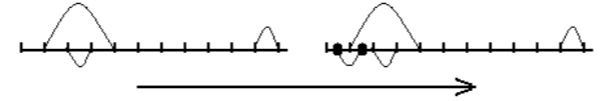
\includegraphics[scale=0.8]{teleport.png}

На первом рисунке показан отрезок с тремя заданными телепортами. На втором рисунке показан тот же отрезок после добавления
нового телепорта, соединяющего точки 0.5 и 1.5.

В первом примере, после добавления нового телепорта способом, показанным на рисунке, вы сможете путешествовать следующим образом: :
\begin{itemize}
\item Вы стартуете с позиции 0 и двигаетесь на восток. 
\item Вы достигаете точки телепорта в позиции 0.5 и телепортируетесь в позицию 1.5
(зарабатывается 1 балл). 
\item Вы продолжаете двигаться на восток и достигаете точки телепорта в позиции 2; вы
телепортируетесь в позицию 3 (у вас 2 балла). 
\item Вы достигаете точки телепорта в позиции 4 и телепортируетесь в позицию 1 (у вас 3 балла). 
\item Вы достигаете точки телепорта в позиции 1.5 и телепортируетесь в позицию 0.5 (у вас 4
балла). 
\item Вы достигаете точки телепорта в позиции 1 и телепортируетесь в позицию 4 (у вас 5 баллов). 
\item Вы достигаете точки телепорта в позиции 10 и телепортируетесь в позицию 11 (у вас 6
баллов). 
\item Вы продолжаете двигаться и достигаете конца отрезка с общей суммой в 6 баллов. 
\end{itemize}